\chapter{Landshark description}
This chapter provides a brief description of the components and configuration of the Phase 2
Landshark system.

\section{Hardware components}

The Landshark system consists of two parts: the Landshark robot with the blackbox computer and
the OCU with a tablet computer. This configuration is a ``thin'' version and not all the
components are used.
The OCU tablet has the following external hardware.  The tablet runs Ubuntu 14.04.
\begin{itemize}
  \item XBox wired controller (USB)
  \item Radio (NIC)
  \item Optional keyboard and mouse (USB).
\end{itemize}
The blackbox has the following hardware components for Phase 2.  
\begin{itemize}
  \item Radio (NIC)
  \item US Digital USB4 controller (USB)
  \item IP-based turret controller (USB NIC)
  \item IP-based paintball trigger (USB NIC)
  \item MOOG controller\footnote{This does not work due to firmware issues} (serial port) 
  \item 2 Hokuyo lasers (USB)
  \item 2 Microstrain IMUs (USB)
  \item 1 GPS device (USB)
\end{itemize}
The blackbox runs the Certikos Hypervisor with 5 VMs. All the VMs run Ubuntu 14.04.

\section{Blackbox VM description}
The VMs running on the blackbox are described below.
\begin{itemize}
  \item VM1 (Communication): The built-in NIC is connected to this VM. This VM has a static IP
    address of {192.168.45.69}. It is connected to the same network as the OCU tablet via the radio link.
    This VM runs nodes that relay messages between the OCU and the other VMs. The communication
    between VM1 and the OCU uses IP packets (Kestrel protocol). Inter-VM and intra-VM communication 
    is performed using shared memory (Kestrel protocol) provided by Certikos.
  \item VM2 (Driver): The USB ports in the back of the blackbox and serial port are
    connected to this VM. All sensor, actuator devices are connected to this VM through the 
    above ports. The driver
    nodes and the FSM node run on this VM. The IP devices (turret, paintball gun) are
    connected to this VM through a USB NIC (DHCP address on the internal robot network
    {192.168.15.0}). 
  
  \item VM3 (CMU): The CMU controllers and monitor nodes run on this VM. No hardware is
    connected to this VM. (Only the \emph{stub} versions are provided in this release as the
    actual controllers and components have not been integrated and tested.)
  \item VM4 (UPenn): The Univ. of Penn. CCC and RSE nodes run on this VM. No hardware is
    connected to this VM.
  \item VM5 (Red Team): This VM has access to the front USB ports. A USB NIC can be plugged
    into this VM and it is configured to have a static IP address of {192.168.1.10}. On
    rebooting, the udev rule 70-persistent-net.rules file is deleted. It is
    advisable to use the same USB NIC in a session so that the network interfaces on Linux is
    configured correctly and gets the appropriate IP address. You may SSH into this VM using the
    username \texttt{hacms} and the password \texttt{hackme}.
\end{itemize}


\section{Network configuration}

The blackbox (VM1) is connected through the radio to the OCU. The OCU and VM1 are in the
private 192.168.45.0 network and have static IP addresses. The IP-based devices and VM2 are
connected to the 192.168.15.0 private network on the Landshark. VM5 has USB ports and is
configured to have a static IP on the 192.168.1.0 network. The network configuration is
illustrated in Table~\ref{tab:network}.

The OCU and VM1 have IPSec and Linux firewall configured to accept packets only from each other.

The radio encryption is turned off by default for the convenience of the Red Team as they have
indicated in the past that it is not the focus of the program. 

\begin{table}
\footnotesize
\begin{tabular}{ |c|c|c|c|c|c| } \hline
  Machine & Device & Name & Network & IP address & connected to \\ \hline
  OCU & NIC & eth0 & 192.168.45.0 & 192.168.45.89 & Radio \\ 
  VM1 & NIC & eth0 & 192.168.45.0 & 192.168.45.69 & Radio \\ 
  VM2 & USB NIC & eth0 & 192.168.15.0 & DHCP & IP devices \\ 
  VM3 & & & & &  \\ 
  VM4 & & & & &  \\ 
  VM5 & USB NIC & eth0 & 192.168.1.0 & 192.168.1.10 & Red Team network \\ 
  \hline
\end{tabular}
\caption{Network configuration on the Landshark system}
\label{tab:network}
\end{table}

\section{Device configuration}
Cables on the blackbox should be connected as described below. The blackbox back and front ports
are illustrated in Figures~\ref{fig:blackbox_front} and \ref{fig:blackbox_back}.
The blue ethernet cable labeled radio should go into the NIC on the blackbox. 
The USB cables labeled ``GPS'', ``US Digital'', ``9 Port USB HUB'' and the USB NIC should go in the USB ports A and B. 
USB ports C should not have anything plugged in them.
USB ports D may have keyboard and USB NIC for red team plugged in. They will be accessed by VM5.

\begin{figure}[htb]
\begin{center}
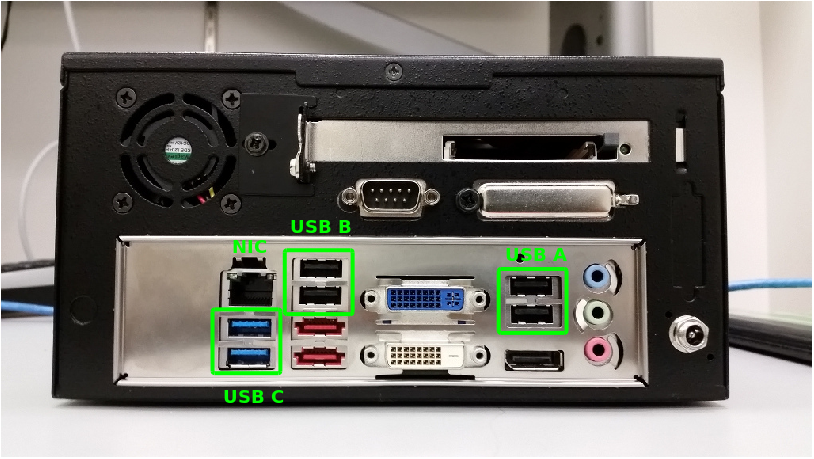
\includegraphics[height=60mm]{figures/blackbox_back.png}
\caption{Blackbox back}
\label{fig:blackbox_back}
\end{center}
\end{figure}

\begin{figure}[htb]
\begin{center}
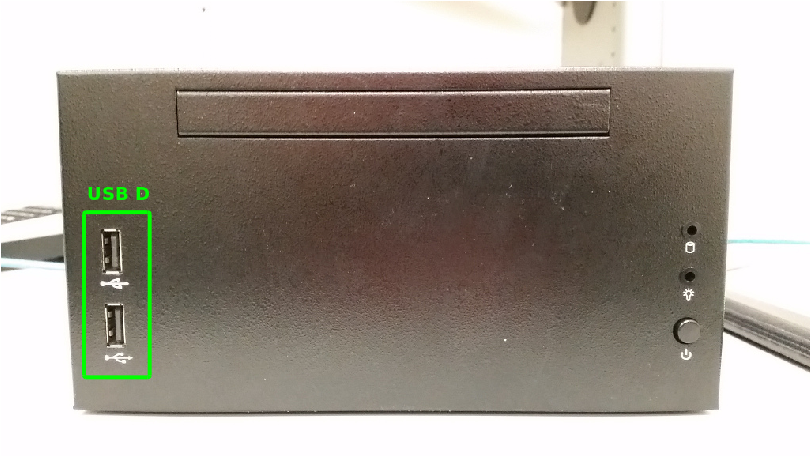
\includegraphics[height=60mm]{figures/blackbox_front.png} 
\caption{Blackbox front}
\label{fig:blackbox_front}
\end{center}
\end{figure}



\chapter{Software description}
The software has been written using the Robot Architecture Description Language (RADL). The system
consists of the following classes of nodes. 
\begin{itemize}
  \item User Interface (UI) nodes (XBox controller, OCU GUI)
  \item Gateway nodes relaying messages between the OCU and blackbox 
  \item Drivers for the various sensors and actuators
  \item Control FSM for selecting and multiplexing the base controllers
  \item Autonomous and semi-autonomous controllers (CCC, PP) for the base
  \item Monitors that estimate system state and flag warnings
\end{itemize}

\section{Control FSM}
\label{sec:fsm}

The FSM dictates how control is coordinated amongst the different controllers and 
is responsible for sending the appropriate actuator value to the BASE node. 
Figure~\ref{fig:fsm_radl} shows part of the RADL architecture containing the FSM node 
and the nodes connected to it.

\begin{figure}[ht]
  \centering
  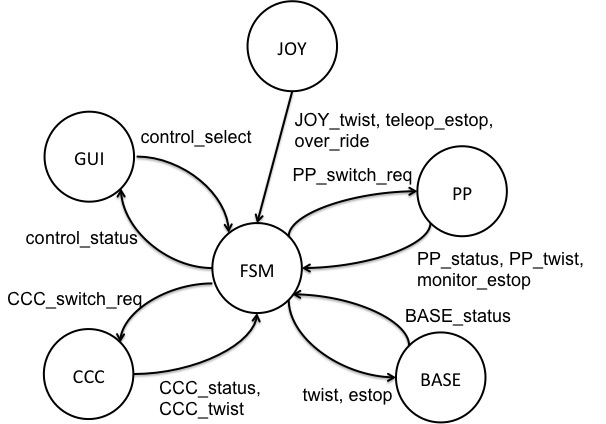
\includegraphics[width=0.7\textwidth]{figures/fsm_radl.jpg}
  \caption{The FSM arbitrates the switch amongst the three controllers -- Constant Cruise Controller (CCC), Path Planner (PP) and Joystick (JOY). Based on the arbitration result, it then sends the appropriate twist (linear and angular velocity) message to the BASE node.}
  \label{fig:fsm_radl}
\end{figure}

There are currently 5 RADL nodes connected to the FSM. 
Among these, CCC, PP and JOY are the controllers, each producing its own twist message. 
CCC and PP are autonomous controller and JOY corresponds to manual input generated by a user operating the joystick. 
During normal operation, the user can select a controller to control the vehicle by setting the \texttt{control\_select} signal from the GUI.
The FSM may also receive a \texttt{ESTOP} message in a scenario where emergency stop is required.  
Currently, there are two \texttt{ESTOP} messages -- one produced by the monitor (\texttt{monitor\_estop}) 
and sent to the FSM through the PP node, and the other from the joystick (\texttt{teleop\_estop}). 
Hence, the FSM maintains 4 control modes -- \texttt{CCC}, \texttt{PP}, \texttt{JOY} and \texttt{ESTOP}. 
The FSM also publishes its current control mode through the \texttt{control\_status} message to the GUI. 
Depending on which control mode it is in, the FSM forwards the corresponding twist message to the BASE. 
For instance, if the FSM is in \texttt{CCC} mode, then it sets \texttt{twist} to \texttt{CCC\_twist}. 
%In addition, if it receives a \texttt{ESTOP} message in this mode, then it will also forward it to the BASE.
The \texttt{over\_ride} message behaves in a similar way as a control select on the joystick -- when it is set, 
the FSM should switch to the \texttt{JOY} mode as soon as possible. 

\noindent
{\bf Control priority.}
Control priority determines the conditions under which the FSM should switch to a particular mode. 
Manual control always supersedes other control modes. Note that this also means the user can use the joystick to move the vehicle
when it is in the \texttt{ESTOP} mode. 
\texttt{ESTOP} has a higher priority than any of the two auto modes but a lower priority than manual control. 
This means the \texttt{ESTOP} mode can be entered when the FSM is currently in one of the two auto modes (\texttt{CCC} or \texttt{PP}) and 
receives a \texttt{teleop\_estop} message set to true (currently \texttt{monitor\_estop} only takes effect when the FSM is in the \texttt{PP} mode).
In addition, the FSM can enter the \texttt{ESTOP} mode if it receives a \texttt{teleop\_estop} message in the \texttt{JOY} mode
(given that the joystick is not selected simultaneously either through the \texttt{control\_select} signal or through setting the 
\texttt{over\_ride} message). 
The two auto modes have equal priority. This means if the FSM is in \texttt{CCC} mode, then it cannot directly jump to the \texttt{PP} mode 
and vice versa. Figure~\ref{fig:fsm_mode} shows the possible transitions among the 4 modes. 

\begin{figure}[ht]
  \centering
  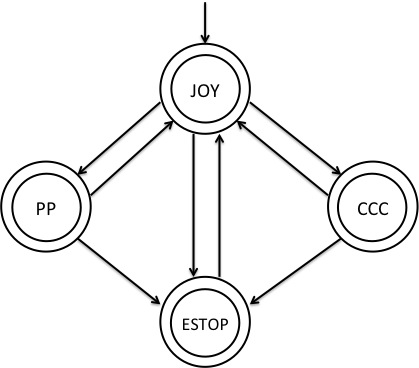
\includegraphics[width=0.5\textwidth]{figures/fsm_mode.jpg}
  \caption{Possible FSM mode transitions. Initially, the FSM is in JOY mode (manual control).}
  \label{fig:fsm_mode}
\end{figure}

\noindent
{\bf Control handshake.}
When the user selects one of the two auto modes (from the \texttt{JOY} mode), 
the FSM will first perform a handshake with the corresponding controller before control can be established for that controller. 
For instance, if the user tries to set the vehicle to constant speed control by setting \texttt{control\_select}, 
the FSM will first send a request (setting the \texttt{CCC\_switch\_req} message to appropriate value) to CCC. 
It then waits for an engage signal (the \texttt{CCC\_status} will be set to \texttt{ENGAGE\_GUARANTEE} or 
\texttt{ENGAGE\_NO\_GUARANTEE}) from the CCC controller for a small number of periods (e.g., $3$). 
If it receives the engage signal within the waiting time, the FSM will transition to the \texttt{CCC} control mode and set the 
actuator output to the BASE (\texttt{twist}) to the value computed by the CCC controller (\texttt{CCC\_twist}) in the same period. 
Otherwise, it stays in the \texttt{JOY} control mode. 



\chapter{Normal Operation}
This chapter describes the normal operation of the robot. 

\section{Starting the robot}
The robot can be powered on by releasing the EStop and pressing the power button on the
blackbox. Certikos boots up first followed by the 5 VMs. The robot nodes start up automatically
in each VM. You may plug in an USB NIC to gain SSH access to VM5. 
There is a master power button on the side of the robot which should be turned on as well.

\section{Shutting down the robot}
The robot should be stopped by shutting down Certikos, followed by a short wait (15 seconds)
and pressing the ESTOP button. You may shutdown Certikos from the OCU tablet using the following
command.

\begin{lstlisting}[language=bash]
ssh hacms@192.168.45.69 "./shutdownall"
\end{lstlisting}

\section{Starting the OCU}
The OCU can be powered on by simply pressing the start button. The power cord needs to be
plugged into an electrical outlet for the radio to function. The OCU nodes start up
automatically as a Linux service. They may be started or stopped using the following commands. 

\begin{lstlisting}[language=bash]
sudo service plant start/stop
\end{lstlisting}

\section{Using the OCU}
The OCU consists of two nodes: \emph{ocu\_teleop} and \emph{ocu\_gui\_server}. There is an
OCU GUI that can be started by clicking on
the shortcut or from a terminal. The GUI is a client for the \emph{ocu\_gui\_server}. The GUI
may be alternatively started using the following command.
\begin{lstlisting}[language=bash]
/opt/hacms/bin/ocu_gui_client
\end{lstlisting}


\subsection{Joystick Control}
The joystick can be used to control the robot wheel motors, the turret and the paintball gun
as shown in Figure~\ref{fig:joystick}. The deadman button must be depressed for any other
operation.

\begin{figure}[htb]
\begin{center}
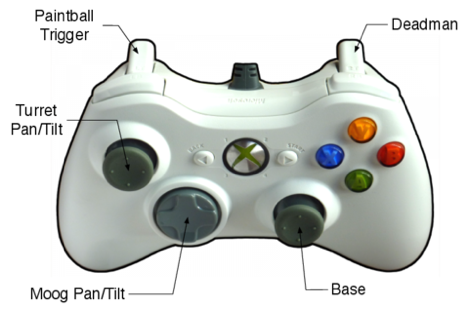
\includegraphics[height=50mm]{figures/joystick.png} 
\caption{Joystick operation}
\label{fig:joystick}
\end{center}
\end{figure}



\subsection{OCU GUI}

The OCU GUI displays the status messages from different nodes on the machine. It is also used to
turn on the CCC (Univ. of Penn. Constant-speed Cruise Control) and PP (CMU Path Planner) modes.
A screenshot of the GUI is provided in Figure~\ref{fig:ocu}. The ``OCU Server connection'' section
shows the status of the communication between the OCU server and client only. It should display
a continuously incrementing ``seq'' value if the OCU plant is running.

The ``Status'' section displays the messages and associated flags from the different VMs on the
OCU and serves as a debug display. If the OCU is communicating correctly, the following messages
should appear. 
\begin{lstlisting}
FSM: stale: v=0, m=0, timeout: v=0, m=0
FSM: stale: v=0, m=0, timeout: v=0, m=0
\end{lstlisting}
The ``seq'' value in the ``Base:'' and ``Actuator:'' lines should also be continuously incrementing. If
this is not the case, one or more of the following may be true.
\begin{itemize}
  \item The blackbox is not up (or is not working)
  \item The radio connection between the blackbox and the OCU is not working.
\end{itemize}

\begin{figure}[htb]
\begin{center}
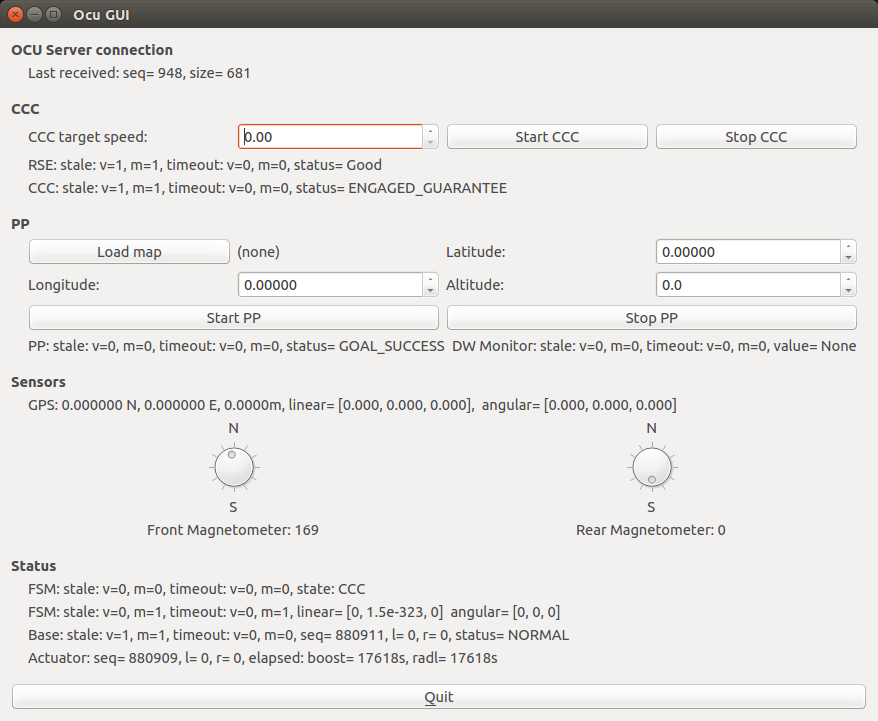
\includegraphics[height=90mm]{figures/ocu.png} 
\caption{OCU GUI (client)}
\label{fig:ocu}
\end{center}
\end{figure}

\subsection{Landshark modes}
The Landshark operates in four modes: JOY, CCC, PP and ESTOP as described in
Section~\ref{sec:fsm}. 

\subsubsection{JOY mode}
This mode is the default manual operation when the XBox controller is in control.

\subsubsection{CCC mode}
In this mode, the landshark moves in a straight line at the user-set speed. The details of this
mode are in a separate document provided along with this manual.

\subsubsection{PP mode}
This mode is not included in this release except as a stub which does nothing. You may switch
into and out of this mode.

\subsubsection{EStop mode}
The user may request the landshark to go into an EStop mode by simultaneously pressing the
``LB'' and ``RB'' buttons on the Xbox controller. You may over-ride this mode by pressing
the ``deadman'' button to go into the JOY mode.

\chapter{Recommended procedures and Troubleshooting}

\section{Recommended procedures}
We recommend that you follow these procedures to avoid common problems.
\begin{enumerate}
  \item If you do not plan to move the robot around and for the first few days of testing the
    robot, please use a motorcycle jack and connect a keyboard and monitor to the blackbox. This
    will enable you to notice common boot problems due to change of boot order, etc. If
    the system boots correctly, it will drop you in a shell for Landshark VM5 (Red Team VM). You
    can configure the network from the console as per your requirement.
    %\emph{You should not connect or disconnect the monitor when Certikos is running.}
  \item Always shut down the blackbox from VM1. If you are forced to shut down the blackbox without
    using the shutdown process, we recommend that you connect a monitor before booting up the
    next time. You may do a file system check on the partitions on the CF card by inserting in a
    different computer.
  \item Always make sure the Landshark is charging when left for more than a couple of hours at a
    time.
  \item Always make sure that there is a valid CF card in the slot before booting the Landshark.
    If the CF card is not present, the boot order will change and the Landshark will not boot
    from the right device subsequently. You will need to set the correct boot order from the
    BIOS in this case.
\end{enumerate}


\section{Known issues}
\begin{itemize}
  %\item The monitor should not be plugged or unplugged when Certikos is booted.
  \item Certikos does not boot correctly occasionally.
\end{itemize}


\section{Troubleshooting}

\subsection{The blackbox does not boot}
This will happen if an attempt is made to boot the blackbox without a CF card. The BIOS will
change the default boot option to SSD. 

\subsubsection{How to check}
If the Landshark boots up correctly and the base is operational, the LED at the left rear part
of the Landshark will blink at approximately 1Hz. You may also attach a monitor before booting
to view the output of the boot process. If Certikos boots correctly, you should be presented
with a VM5 console in approximately one minute. 

\subsubsection{How to fix}
To fix this, the BIOS should be changed to reorder the
boot order so that the CF card is the first boot device.

\subsection{Certikos does not boot}
This may happen occasionally and is a known issue. 

\subsubsection{How to check}
If the Landshark boots up correctly and the base is operational, the LED at the left rear part
of the Landshark will blink at approximately 1Hz. You may also attach a monitor before booting
to view the output of the boot process. If Certikos boots correctly, you should be presented
with a VM5 console in approximately one minute. 

\subsubsection{How to fix}
To fix this, turn off the blackbox and restart.

\subsection{The OCU cannot communicate with the Landshark}
The radio does not work sometimes. 

\subsubsection{How to check}
You can check using the GUI if the OCU is receiving messages from the Landshark. For the FSM,
you should see ``mbox=0''. If the base node is also working correctly, you should see the sequence
number constantly being incremented in rows 3 and 4. You should also be able to ping and ssh
into VM1 (192.168.45.69) from the OCU.

\subsubsection{How to fix}
This can usually be fixed by rebooting the radio on the OCU side.

\section{Manual control}
You may use a second CF card labeled ``BACKUP'' to move the robot. This a bare-bones version (not
HA) that is useful for trouble-shooting the robot and joysticking the robot around without using
the radio or HA components. If you use this CF card, you have to plug in a wired XBox controller to any USB port on the blackbox. You do not need the OCU.

\section{BIOS settings}
If you wish to boot an identical blackbox with the CF card, you will need to use the following
settings in the BIOS.

\begin{itemize}
  \item USB Legacy is disabled.
  \item USB 3.0 Controllor and all USB ports are enabled.
  \item Boot hard drive order with CF card being the first one.
\end{itemize}


\chapter{Red Team Attack Surface}
\label{sec:attack}

The HACMS landshark system has been designed to prevent certain kinds of attacks. These are
listed in Section~\ref{sec:attack-protected}.  Some aspects of the system have not yet been
covered and are out of scope.
These are listed in Section~\ref{sec:attack-out-of-scope}. 

The red team will have access to the following to attempt to break into the Landshark or disrupt
communication.
\begin{enumerate}
  \item	Wireless radio communication between the Operator’s Control Unit (OCU) and the
    LandShark.
  \item	Full access to VM5, one of the 5 virtual machines running on the Black Box under
    Certikos including the USB ports on the front of the blackbox.
\end{enumerate}

\section{Protected components}
\label{sec:attack-protected}
This section lists the protected components of the system. 
\begin{enumerate}
  \item The communication between VM1 and the OCU has been secured using IPsec and Linux
    firewall.
    \begin{enumerate}
      \item This should prevent spoofing of the OCU or VM1 by attackers.
      \item This should prevent replay attacks.
    \end{enumerate}
  \item The communication between different VMs using the Kestrel stack using shared memory
    protected by Certikos.
  \item The system should be resilient to unplugging or spoofing one (and only one) of the following sensors
    \begin{enumerate}
      \item GPS
      \item Left side odometry
      \item Right side odometry
    \end{enumerate}
  %\item	Denial of Service (DoS) attacks over the radio?
  %\item	Denial of Service (DoS) attacks on a mailbox?
\end{enumerate}


\section{Unprotected components (out of scope)}
\label{sec:attack-out-of-scope}
The following things are not yet protected, so they are out of scope.
The red team may not attack the landshark system in the following ways.
\begin{enumerate}

  \item You may not modify the CF card except inside partition 13 (the Red Team VM).
  \item You may not read the IPSec private key stored in the partition 5 of the CF.
  \item	You may not attack the OCU. You may, however, try to spoof the IP packets from VM1 to the OCU.
  \item	You may not plug in any device in the back of the blackbox. 
  \item	You may not turn off power to the blackbox.
  \begin{enumerate}
    \item The firmware (specifically in the base controller) has not been protected. If the
      blackbox is powered off, it will keep moving (if it was moving at the time of the
      poweroff).
    \item This may corrupt the CF card.
  \end{enumerate}
\end{enumerate}



